\documentclass[hidelinks,12pt,dvipsnames,border=2pt]{standalone}
%\usepackage[top=0.7in, bottom=0.8in, left=1in, right=1in]{geometry}
\usepackage{tikz}
\usepackage{hyperref}
\usetikzlibrary{arrows}
\usetikzlibrary{shapes}
\usepackage{enumitem}
\usepackage{bm}
\usepackage{mathdots}
\usepackage{amsmath}
\usepackage{tcolorbox}
\usetikzlibrary{shadings}
\usetikzlibrary{decorations.pathreplacing}
\usepackage{helvet}
\usepackage{url}
\usepackage{graphicx}
\usetikzlibrary{arrows.meta,positioning,fit,calc}
\renewcommand{\familydefault}{\sfdefault}


\usetikzlibrary{arrows,decorations.pathmorphing,backgrounds,fit,positioning,shapes.symbols,chains}

\begin{document}
	
% trim=left botm right top
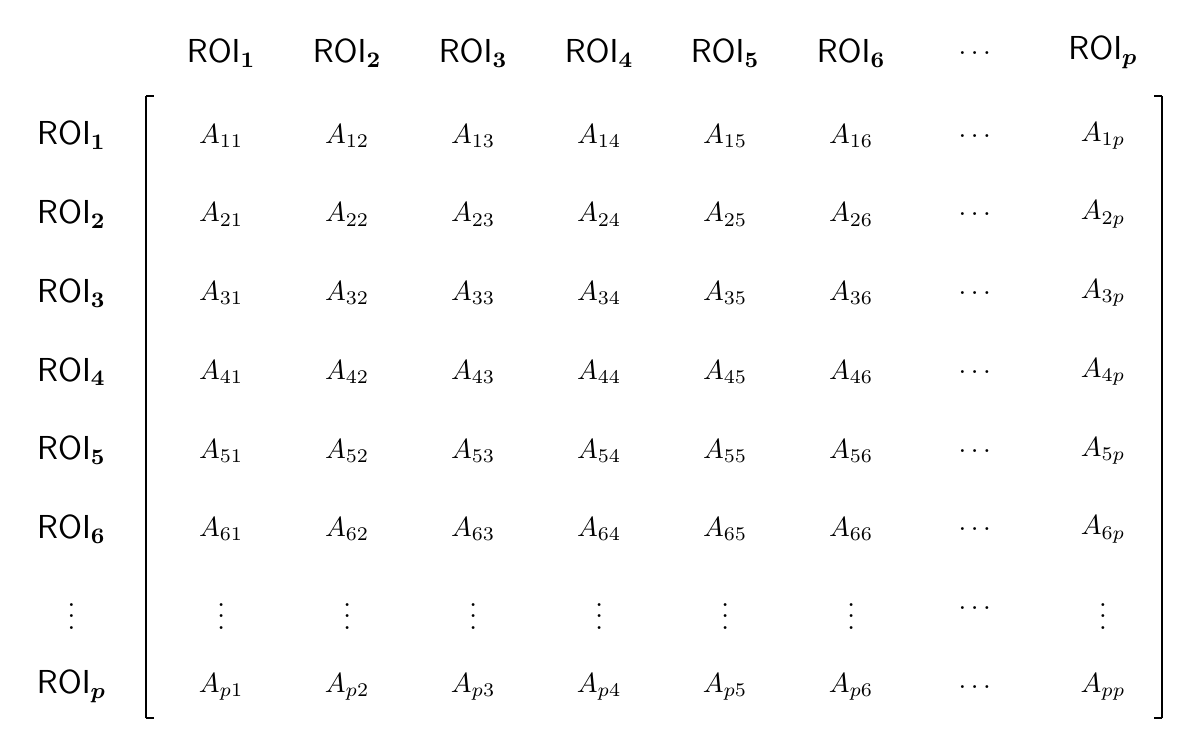
\begin{tikzpicture}
\node at (0,-0.45) {\large \bm{$\text{ROI}_1$}};
\node at (1.6,-0.45) {\large \bm{$\text{ROI}_2$}};
\node at (3.2,-0.45) {\large \bm{$\text{ROI}_3$}};
\node at (4.8,-0.45) {\large \bm{$\text{ROI}_4$}};
\node at (6.4,-0.45) {\large \bm{$\text{ROI}_5$}};
\node at (8,-0.45) {\large \bm{$\text{ROI}_6$}};
\node at (9.6,-0.45) {$\dots$};
\node at (11.2,-0.45) {\large \bm{$\text{ROI}_p$}};

%\draw [decorate,decoration={brace,amplitude=25pt,aspect=0.5},xshift=-4pt,yshift=0pt,line width=0.4mm,draw=cyan] (-0.25,0) -- (11.5,0) node [black,xshift=9pt] {\footnotesize};
%\node at (5.5,1.35) {\Large Instances};

\node at (-1.9,-1.5) {\large \bm{$\text{ROI}_1$}};
\node at (-1.9,-2.5) {\large \bm{$\text{ROI}_2$}};
\node at (-1.9,-3.5) {\large \bm{$\text{ROI}_3$}};
\node at (-1.9,-4.5) {\large \bm{$\text{ROI}_4$}};
\node at (-1.9,-5.5) {\large \bm{$\text{ROI}_5$}};
\node at (-1.9,-6.5) {\large \bm{$\text{ROI}_6$}};
\node at (-1.9,-7.5) {$\vdots$};
\node at (-1.9,-8.5) {\large \bm{$\text{ROI}_p$}};

%\draw [decorate,decoration={brace,amplitude=25pt,aspect=0.5,mirror},xshift=-4pt,yshift=0pt,line width=0.4mm,draw=cyan] (-1.95,-1) -- (-1.95,-9.95) node [black,xshift=9pt] {\footnotesize};
%\node at (-4,-5.475) {\Large SNPs};

% row 1
\node at (0,-1.5) {$A_{11}$};
\node at (1.6,-1.5) {$A_{12}$};
\node at (3.2,-1.5) {$A_{13}$};
\node at (4.8,-1.5) {$A_{14}$};
\node at (6.4,-1.5) {$A_{15}$};
\node at (8,-1.5) {$A_{16}$};
\node at (9.6,-1.5) {$\dots$};
\node at (11.2,-1.5) {$A_{1p}$};

% row 2
\node at (0,-2.5) {$A_{21}$};
\node at (1.6,-2.5) {$A_{22}$};
\node at (3.2,-2.5) {$A_{23}$};
\node at (4.8,-2.5) {$A_{24}$};
\node at (6.4,-2.5) {$A_{25}$};
\node at (8,-2.5) {$A_{26}$};
\node at (9.6,-2.5) {$\dots$};
\node at (11.2,-2.5) {$A_{2p}$};

% row 3
\node at (0,-3.5) {$A_{31}$};
\node at (1.6,-3.5) {$A_{32}$};
\node at (3.2,-3.5) {$A_{33}$};
\node at (4.8,-3.5) {$A_{34}$};
\node at (6.4,-3.5) {$A_{35}$};
\node at (8,-3.5) {$A_{36}$};
\node at (9.6,-3.5) {$\dots$};
\node at (11.2,-3.5) {$A_{3p}$};

% row 4
\node at (0,-4.5) {$A_{41}$};
\node at (1.6,-4.5) {$A_{42}$};
\node at (3.2,-4.5) {$A_{43}$};
\node at (4.8,-4.5) {$A_{44}$};
\node at (6.4,-4.5) {$A_{45}$};
\node at (8,-4.5) {$A_{46}$};
\node at (9.6,-4.5) {$\dots$};
\node at (11.2,-4.5) {$A_{4p}$};

% row 5
\node at (0,-5.5) {$A_{51}$};
\node at (1.6,-5.5) {$A_{52}$};
\node at (3.2,-5.5) {$A_{53}$};
\node at (4.8,-5.5) {$A_{54}$};
\node at (6.4,-5.5) {$A_{55}$};
\node at (8,-5.5) {$A_{56}$};
\node at (9.6,-5.5) {$\dots$};
\node at (11.2,-5.5) {$A_{5p}$};

% row 6
\node at (0,-6.5) {$A_{61}$};
\node at (1.6,-6.5) {$A_{62}$};
\node at (3.2,-6.5) {$A_{63}$};
\node at (4.8,-6.5) {$A_{64}$};
\node at (6.4,-6.5) {$A_{65}$};
\node at (8,-6.5) {$A_{66}$};
\node at (9.6,-6.5) {$\dots$};
\node at (11.2,-6.5) {$A_{6p}$};

% row dots
\node at (0,-7.5) {$\vdots$};
\node at (1.6,-7.5) {$\vdots$};
\node at (3.2,-7.5) {$\vdots$};
\node at (4.8,-7.5) {$\vdots$};
\node at (6.4,-7.5) {$\vdots$};
\node at (8,-7.5) {$\vdots$};
\node at (9.6,-7.5) {$\dots$};
\node at (11.2,-7.5) {$\vdots$};

% row dots
\node at (0,-8.5) {$A_{p1}$};
\node at (1.6,-8.5) {$A_{p2}$};
\node at (3.2,-8.5) {$A_{p3}$};
\node at (4.8,-8.5) {$A_{p4}$};
\node at (6.4,-8.5) {$A_{p5}$};
\node at (8,-8.5) {$A_{p6}$};
\node at (9.6,-8.5) {$\dots$};
\node at (11.2,-8.5) {$A_{pp}$};

\draw[line width=0.25mm] (-0.95,-8.9) -- (-0.95,-1);
\draw[line width=0.25mm] (-0.95,-1) -- (-0.85,-1);
\draw[line width=0.25mm] (-0.95,-8.9) -- (-0.85,-8.9);

\draw[line width=0.25mm] (11.95,-8.9) -- (11.95,-1);
\draw[line width=0.25mm] (11.95,-1) -- (11.85,-1);
\draw[line width=0.25mm] (11.95,-8.9) -- (11.85,-8.9);
\end{tikzpicture}

\end{document}